\documentclass[11pt,a4paper]{article}

% PAQUETES
\usepackage[T1]{fontenc}%
\usepackage[utf8]{inputenc}%

\usepackage[english]{babel}
\usepackage{amsmath}
\usepackage{amsthm}
\usepackage{amsfonts}
\usepackage[%left=1.54cm,right=1.54cm,top=1.54cm,bottom=1.54cm
    margin=1in,
]{geometry}
\usepackage{xfrac}  
\usepackage{tikz-cd}
\usepackage{enumerate}
\usepackage{amsfonts}
\usepackage{amssymb}
\usepackage{tcolorbox}
\usepackage{rotating}
\usepackage{mathpazo}
% \usepackage{charter}
\usetikzlibrary{babel}
\usepackage{listings}
\usepackage{amssymb}
\usepackage{extarrows}
\usepackage{makeidx}
\usepackage{graphicx}
\usepackage{multirow}
\usepackage{tikz-cd}
\usepackage{tasks}
\usepackage{xcolor}

% Christian
\usepackage{enumitem,etoolbox,titlesec}


%OPERADORES

\DeclareMathOperator{\dom}{dom}
\DeclareMathOperator{\cod}{cod}
\DeclareMathOperator{\id}{id}

\newcommand{\red}[1]{\textcolor{red}{#1}}
\newcommand{\C}{\mathbb{C}}
\newcommand{\im}{\text{Im}}
\newcommand{\R}{\mathbb{R}}
\newcommand{\N}{\mathbb{N}}
\newcommand{\Z}{\mathbb{Z}}
\newcommand{\D}{\mathbb{D}}
\newcommand{\B}{\mbox{Ob}}
\newcommand{\M}{\mbox{Mo}}
\newcommand{\del}{\Delta}
\newcommand{\odel}[1]{\left[#1\right]}
\newcommand{\Hom}[1]{\text{Hom}(#1)}
\newcommand{\adel}[1]{\left\lbrace #1 \right\rbrace}
%\renewcommand{\theequation}{\thesection.\arabic{equation}}
\newcommand{\funcion}[5]{%
{\setlength{\arraycolsep}{2pt}
\begin{array}{r@{}ccl}
#1\colon \hspace{0pt}& #2 & \longrightarrow & #3\\
& #4 & \longmapsto & #5
\end{array}}}

\newcommand{\func}[3]{#1\colon  #2  \to  #3}

\newcommand\restr[2]{{% we make the whole thing an ordinary symbol
  \left.\kern-\nulldelimiterspace % automatically resize the bar with \right
  #1 % the function
  \vphantom{\big|} % pretend it's a little taller at normal size
  \right|_{#2} % this is the delimiter
  }}

%ENTORNOS

% \theoremstyle{theorem}
\newtheorem{teo}{Theorem}[section]
\newtheorem{prop}[teo]{Proposition}
\newtheorem{lem}[teo]{Lemma}
\newtheorem{cor}[teo]{Corollary}

\theoremstyle{definition}
\newtheorem{defi}[teo]{Definition}
\newtheorem{rem}{Remark}[teo]
\newtheorem{exa}{Example}
\newtheorem{eje}{Exercise}
\newtheorem{que}{Question}

\newenvironment{sol}
  {\begin{proof}[\textit{Solution}]}
  {\end{proof}}

\titlelabel{\thetitle.\quad}

\def\contador{}
\graphicspath{{./figures/}}
\newcommand{\qand}{\quad\text{and}\quad}
\usepackage{microtype,parskip}
\setlength{\parindent}{15pt}
\linespread{1.15}
\usepackage{hyperref}
\hypersetup{
    colorlinks=true,  
    allcolors=blue,
    pdfproducer={Christian Chávez},
}

\makeatletter
\@ifclassloaded{exam}{
    \footer{}{\thepage}{}
    \renewcommand{\thequestion}{\bfseries\arabic{question}}
    \renewcommand{\solutiontitle}{\noindent\textit{Solution.}\enspace}
    \unframedsolutions
}{}
\makeatother


\newenvironment{theproof}
{
    \renewcommand{\solutiontitle}{}
    \begin{solution}
    \vspace*{-\baselineskip}
    \begin{proof}
}
{
    \end{proof}
    \end{solution}
    \renewcommand{\solutiontitle}{\noindent\textit{Solution.} }
}

\begin{document}

\def\contador{Lesson 4}
\noindent
\begin{minipage}[c]{0.33\textwidth}
    
\includegraphics[scale=0.37]{sello_yachay.png}
\end{minipage}
\begin{minipage}[c]{0.37\textwidth}
    % \centering
    \textbf{\large School of Mathematical and\\ Computational Sciences}\par
    Abstract Algebra
\end{minipage}
~ 
\begin{minipage}[c]{3mm}
    \raggedleft
    \rule[1.5mm]{0.3mm}{15mm}
\end{minipage}
~ 
\begin{minipage}[c]{0.24\textwidth}
    \raggedleft
    Prof. Pablo Rosero\\
    \& Christian Chávez\\
    \contador{}
\end{minipage}

\vspace{1mm}
\noindent\hrulefill

\vspace{3mm}

\section{The dihedral group}

Objects have bilateral
symmetry if they look the same when flipped over (usually in a specific direction, say vertically).
The easiest geometric examples of objects
with both rotational and bilateral symmetry are regular polygons.

\begin{figure}[!htb]
    \centering
    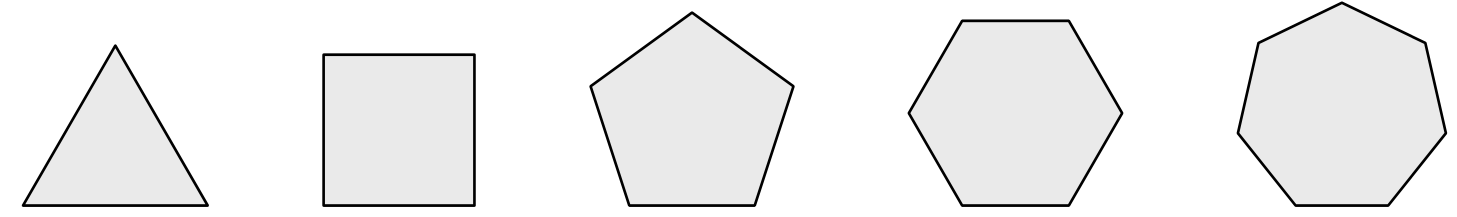
\includegraphics[width=0.75\textwidth]{polygons.png}
    % \caption{}%\label{fig:}
\end{figure}

Observe that is not necessary to track the movement of all the points that make up a  polygon in order to describe a rigid motion. 
Instead, we can simply keep track of their vertices.
This motivates  an important example of groups.

Some definitions first.
A permutation of a set \(X\) is a bijection from \(X\) onto \(X\).
A regular polygon with $n$ sides is called an $n$-gon.
A symmetry of the \(n\)-gon is any rigid motion of of the \(n\)-gon.
To be precise,  a symmetry of the \(n\)-gon is just a permutation of \(\left\{ 1,\ldots, n \right\}\). From now and on, we will denote \([n] = \left\{ 1,\ldots, n \right\}\).

It turns out, we can associate a group to the \(n\)-gon to study its rigid motions, that is, its symmetries.
It is called the dihedral group of order \(2n\) and denoted \(D_{2n}\).
Dihedral groups describe objects that have both rotational and bilateral symmetry.

% For example, 

\begin{exa}
    Both rotations and horizontal flips respect the shape of an equilateral triangle.

\begin{figure}[!htb]
    \centering
    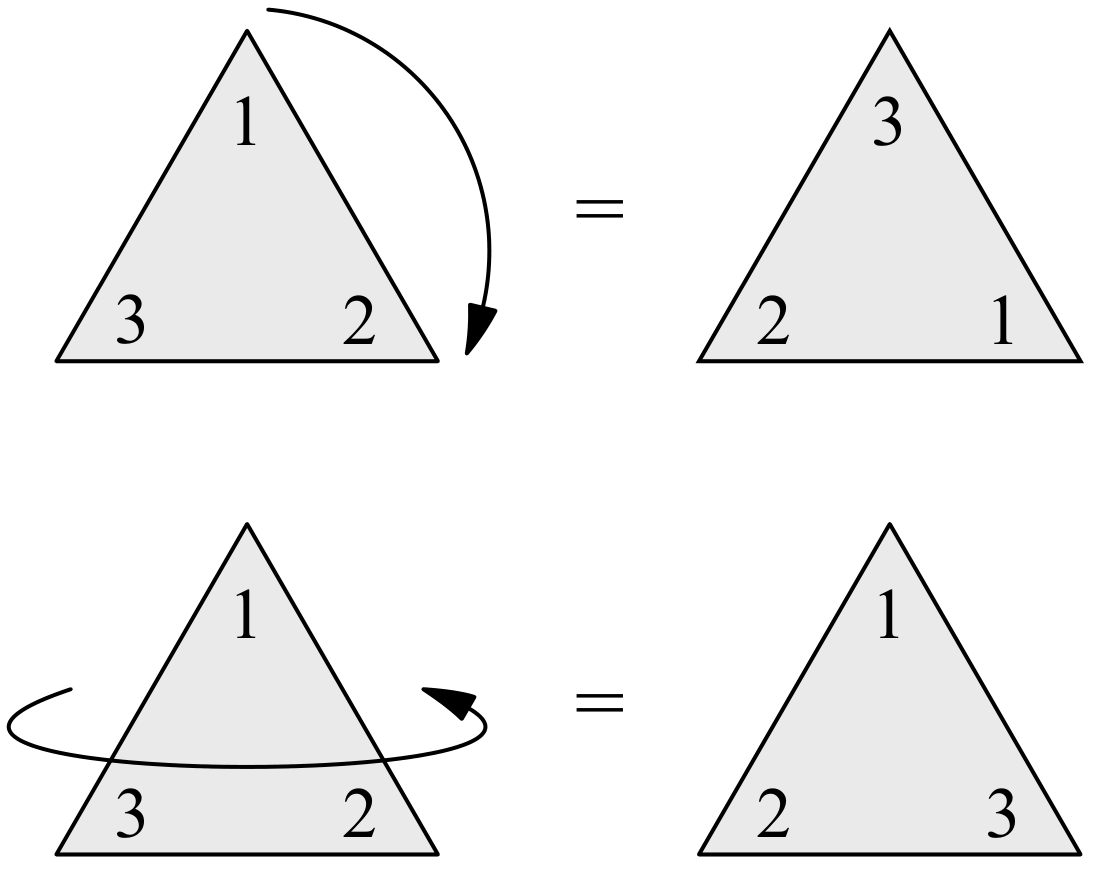
\includegraphics[width=0.3\textwidth]{triangle-rotation.png}
    % \caption{}%\label{fig:}
\end{figure}

The first symmetry is decribed by the permutation \(\sigma\colon [3]\to [3]\) defined by 
\[\sigma(1)=2,\quad\sigma(2)=3,\quad \sigma(3) = 1.\]

The second one is described by \(\tau\colon [3]\to [3]\) where 
\[\tau(1)=1,\quad\tau(2)=3,\quad \tau(3) = 2.\]
\end{exa}

\begin{rem}
    We choose the notation \(D_{2n}\) because there are \(2n\) symmetries associated to a \(n\)-gon. Namely, \(n\) rotations and \(n\) reflections.
\end{rem}

\begin{teo}
\begin{enumerate}[label=(\roman*)]
    \item \(\left\{ 1,r,r^2,\ldots,r^{n-1} \right\}\) are all distinct. Also  \(r^n = 1\) and \(|r| = n\).
    \item \(|s| =2\)
    \item \(s\neq r^i\) for all \(i\in [n]_0\).
    \item \(sr^i = sr^j \) for all \(i,j\in [n-1]\) with \(i\neq j\).
    \item \(rs = sr^{-1}\)
    \item \(r^i s = sr^{-i}\) for all \(0\leq i\leq n\)
\end{enumerate}
\end{teo}

\begin{eje}
    Prove or disprove \((sr^9) (sr^6) = r^9\).
\end{eje}


\section{Permutations and the symmetric group}


\begin{rem}
    \begin{enumerate}[label=(\roman*)]
        \item Not all permutations are cycles.
        \item 
        \item Algorithm to factor a permutation into the product of cycles.
        \item Every permutation has a cycle decomposition.
    \end{enumerate}
\end{rem}


\begin{defi}
    
\end{defi}


\begin{lem}
    Disjoint permutations commute.
\end{lem}


\begin{lem}
    Every permutation of \([n]\) is either a cycle or a product of disjoint cycles.
\end{lem}


\paragraph{}


\end{document}